\cmfnewsection{MMC e Seu Modelo de Pequenos Sinais}{./logos/fundo_tese}{0.15}


%MMC_and_submodules




%%%%%%%%%%%%%%%%%%%%%%%%%%%%%%%%%%%%%%%%%%%%%%%%%%%%%%%
%%%%%%%%%%%%%%%%%%%%%%%%%%%%%%%%%%%%%%%%%%%%%%%%%%%%%%%
%%%%%%%%%%%%%%%%%%%%%%%%%%%%%%%%%%%%%%%%%%%%%%%%%%%%%%%
\begin{frame}{Características do MMC}


\begin{columns}
\column{0.5\textwidth}
\centering
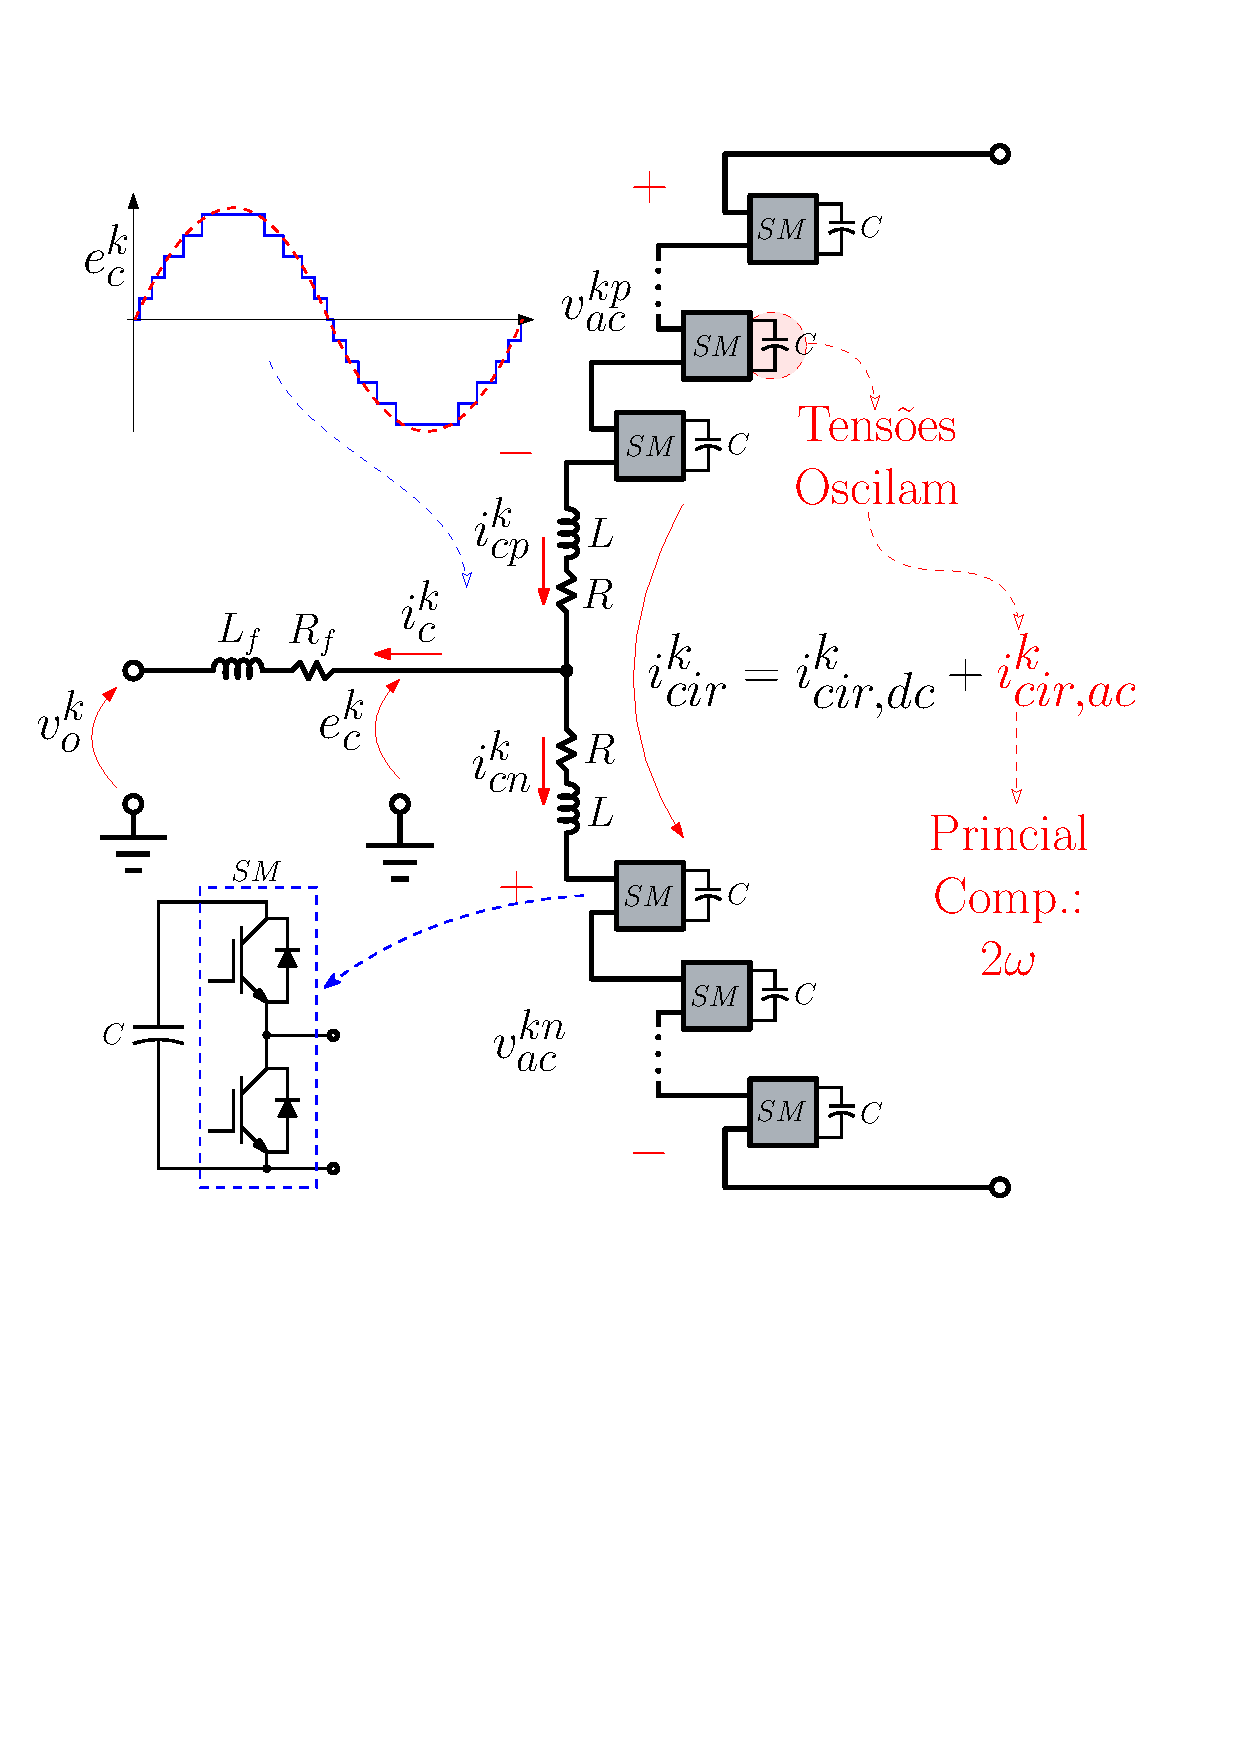
\includegraphics[width=0.9\linewidth]{./figuras/figuras_MMC/MMC_blk_graph3}


\column{0.5\textwidth}

%\centering
Tensão CA
\begin{itemize}
	\item Tem padrão escada\\[5pt]
	\item Depende de quantos SMs são inseridos\\[20pt]
\end{itemize}

Tensões CC
\begin{itemize}
	\item Precisam ser balanceadas\\[5pt]
	\item Têm componentes CC e CA\\[20pt]
\end{itemize}

Corrente Circulante
\begin{itemize}
	\item Tem componentes CC e CA\\[5pt]
	\item Comp. mais sign.: Segundo harmônico 
\end{itemize}

\end{columns}

\end{frame}






%%%%%%%%%%%%%%%%%%%%%%%%%%%%%%%%%%%%%%%%%%%%%%%%%%%%%%%
%%%%%%%%%%%%%%%%%%%%%%%%%%%%%%%%%%%%%%%%%%%%%%%%%%%%%%%
%%%%%%%%%%%%%%%%%%%%%%%%%%%%%%%%%%%%%%%%%%%%%%%%%%%%%%%
\begin{frame}{Acionamento do MMC}

\begin{columns}
\column{0.5\textwidth}
\centering
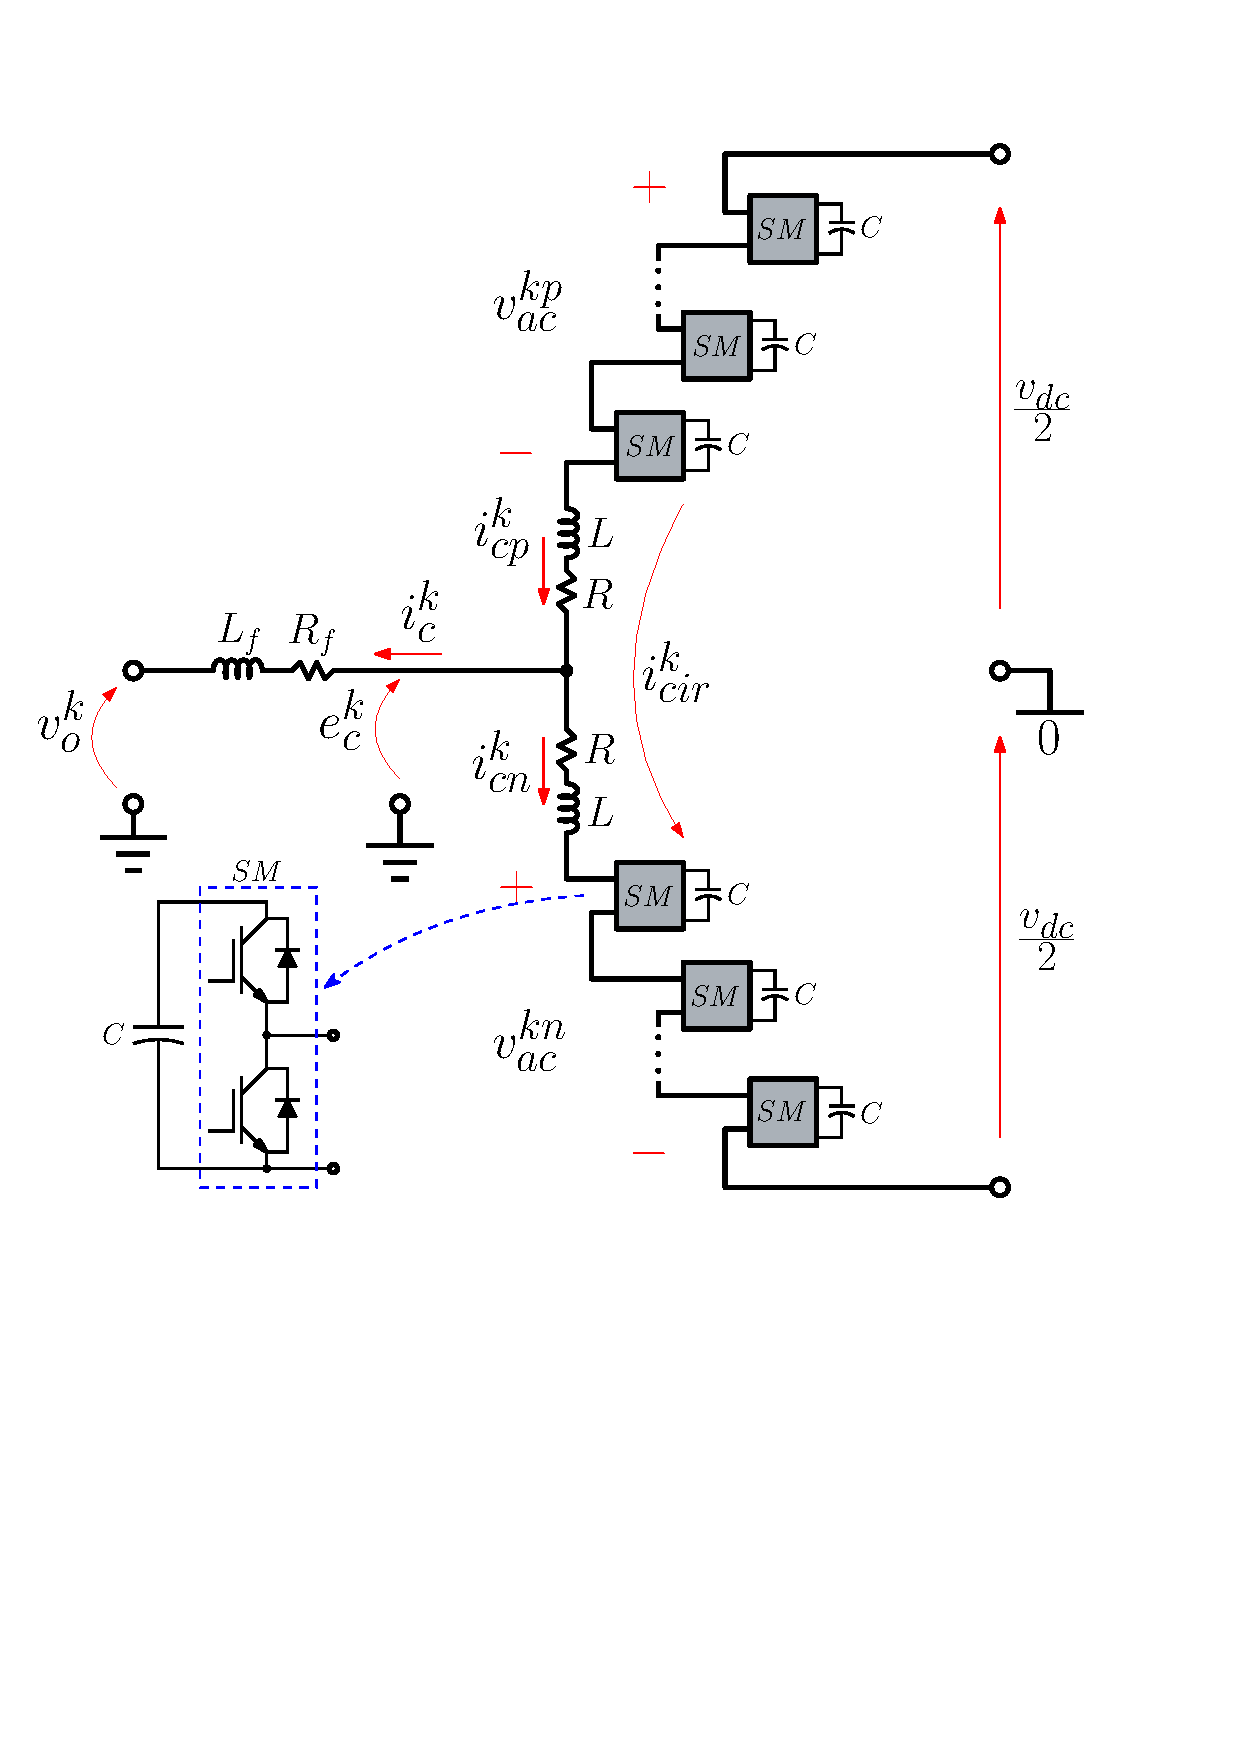
\includegraphics[width=0.9\linewidth]{./figuras/figuras_MMC/MMC_blk}

\column{0.5\textwidth}

\textbf{Índices de Inserção}:
\begin{equation*}
m_{p}^{k}(t) = \frac{1 - e_c^{k*}(t) - e_{cir}^{k*}(t)}{2},
\end{equation*}

\begin{equation*}
m_{n}^{k}(t) = \frac{1 + e_c^{k*}(t) - e_{cir}^{k*}(t)}{2},
\end{equation*}   

\begin{itemize}
	\item Representam quantos SMs são inseridos
\end{itemize}


$e_c^{k*}(t) \mapsto$ Ref. para tensão produzida\\[10pt]


$e_{cir}^{k*}(t)\mapsto$ Atua sobre a corrente circulante

\end{columns}

\end{frame}


%
%%%%%%%%%%%%%%%%%%%%%%%%%%%%%%%%%%%%%%%%%%%%%%%%%%%%%%%%
%%%%%%%%%%%%%%%%%%%%%%%%%%%%%%%%%%%%%%%%%%%%%%%%%%%%%%%%
%%%%%%%%%%%%%%%%%%%%%%%%%%%%%%%%%%%%%%%%%%%%%%%%%%%%%%%%
%\begin{frame}{Conversor e Seu Modelo Médio}
%
%\begin{columns}
%\column{0.5\textwidth}
%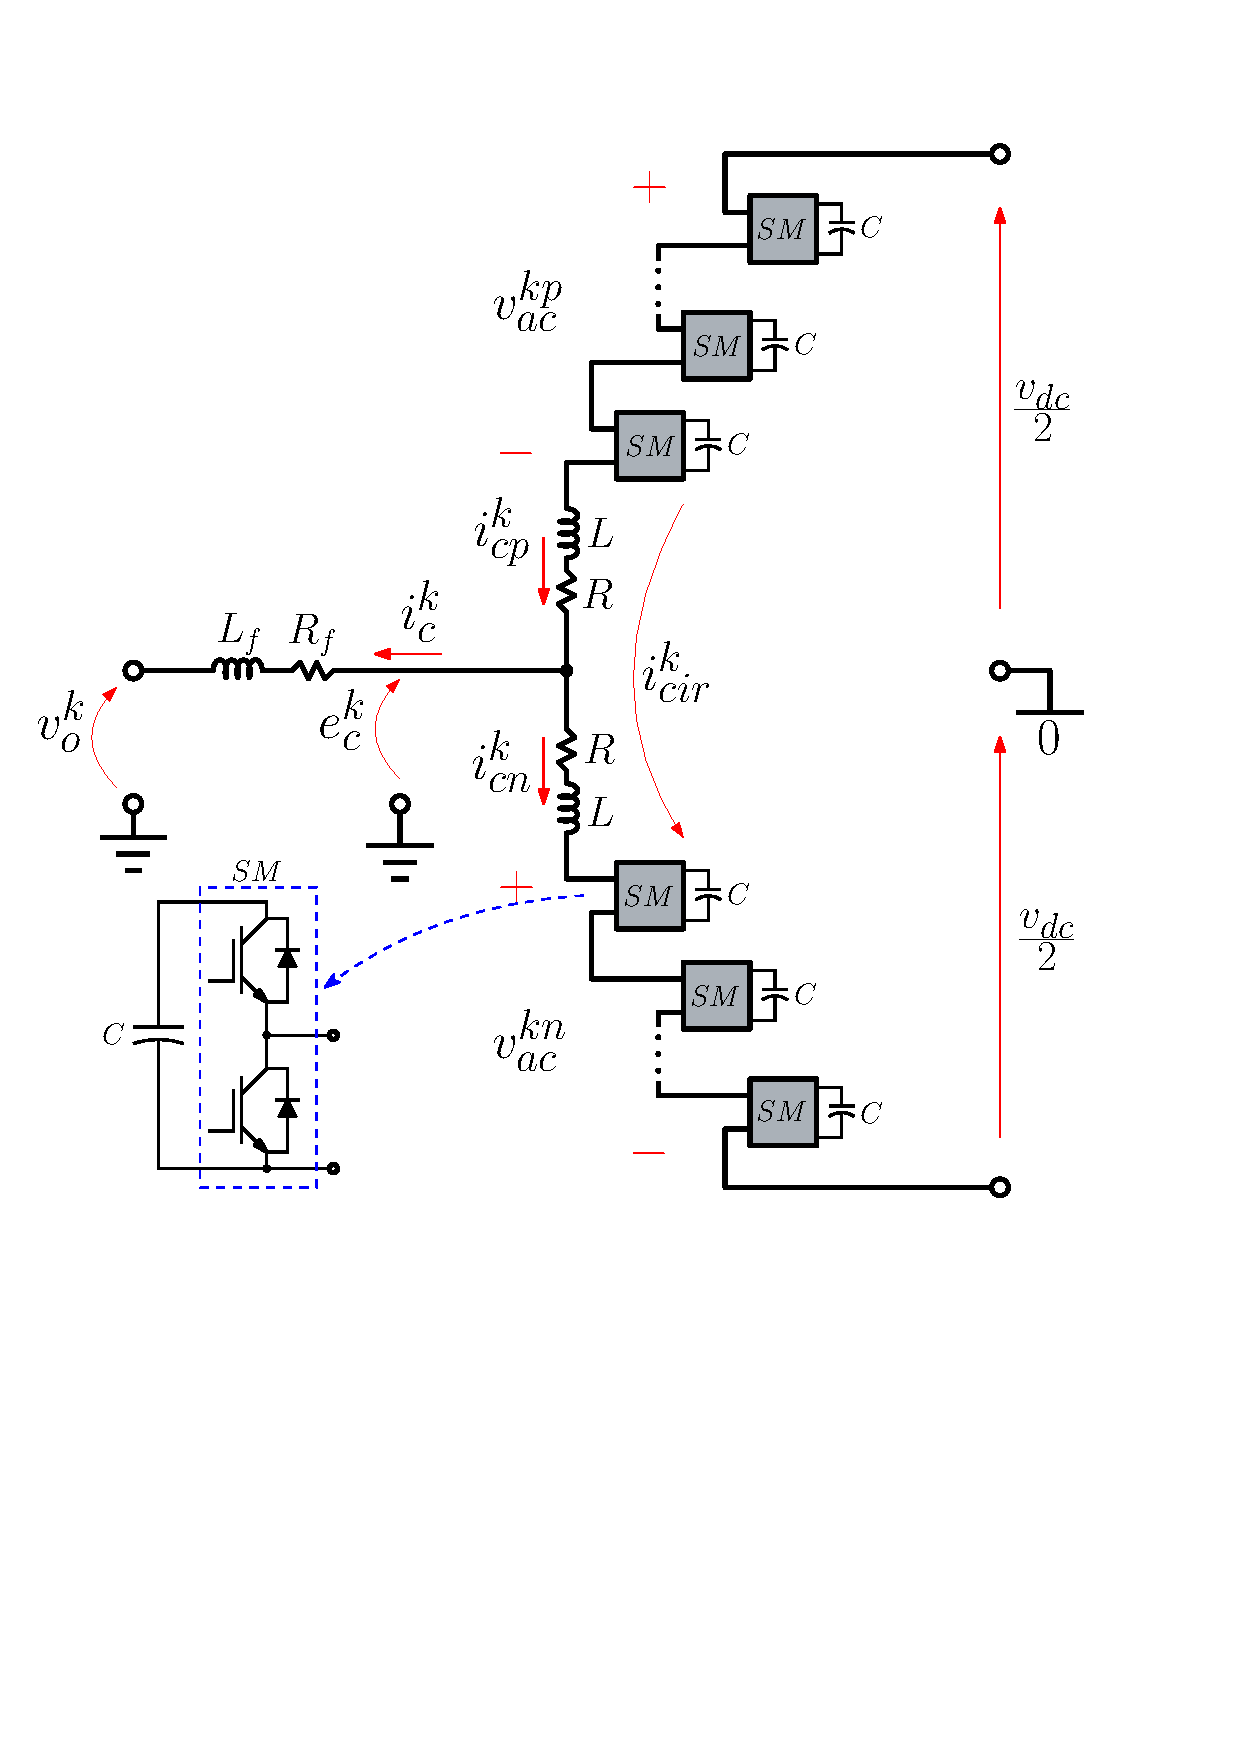
\includegraphics[width=0.9\linewidth]{./figuras/figuras_MMC/MMC_blk}
%\column{0.5\textwidth}
%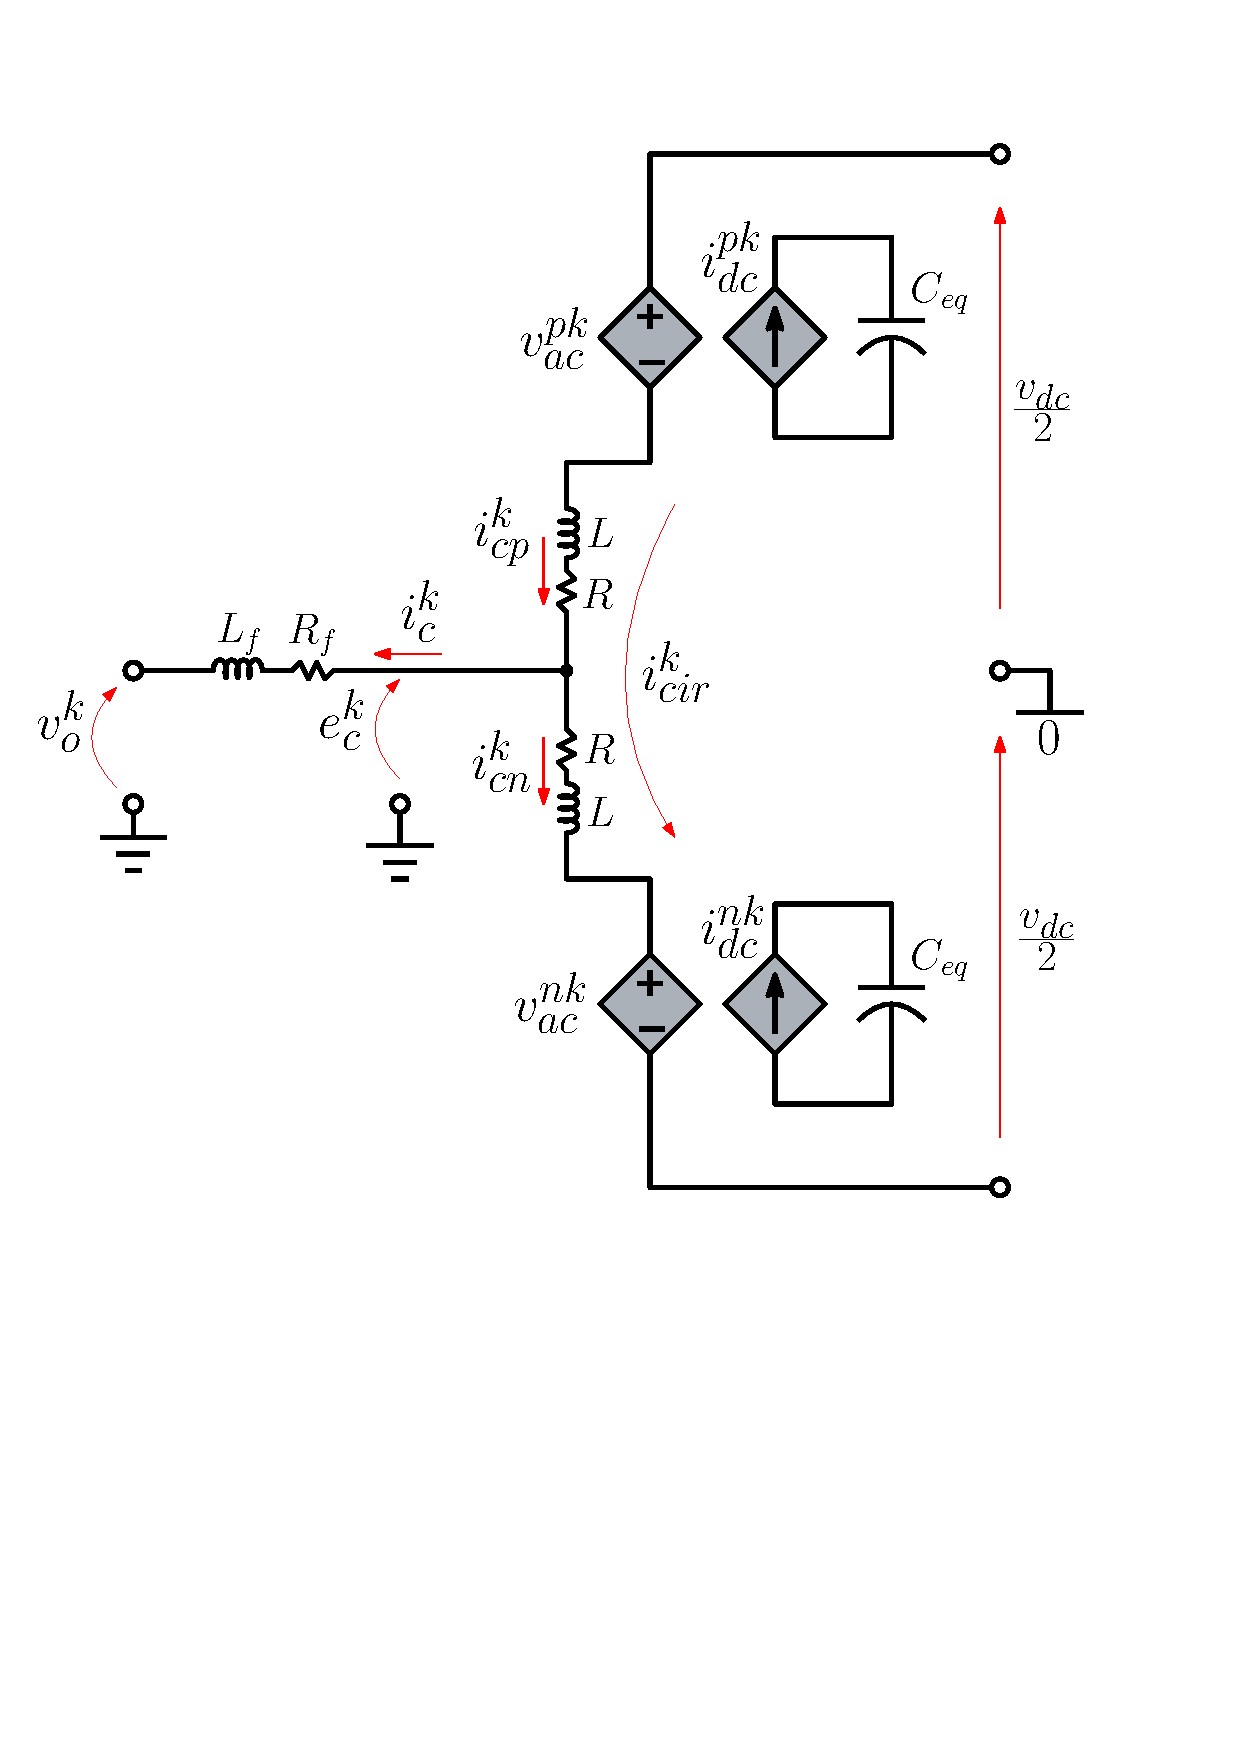
\includegraphics[width=0.9\linewidth]{./figuras/figuras_MMC/MMC_avg}
%\end{columns}
%
%\end{frame}
%
%

%%%%%%%%%%%%%%%%%%%%%%%%%%%%%%%%%%%%%%%%%%%%%%%%%%%%%%%%
%%%%%%%%%%%%%%%%%%%%%%%%%%%%%%%%%%%%%%%%%%%%%%%%%%%%%%%%
%%%%%%%%%%%%%%%%%%%%%%%%%%%%%%%%%%%%%%%%%%%%%%%%%%%%%%%%
%\begin{frame}{Índices de Inserção}
%
%\begin{columns}
%\column{0.5\textwidth}
%
%\begin{itemize}
%	\item Representam quantos SMs são inseridos\\[20pt]
%	\item Foi utilizado uma representação percentual\\[20pt]
%	\item Permitem controlar a tensão produzida\\[20pt]
%	\item Permitem atuar contra a corrente circulante
%\end{itemize}
%
%
%\column{0.5\textwidth}
%
%Índices:
%\begin{equation*}
%m_{p}^{k}(t) = \frac{1 - e_c^{k*}(t) - e_{cir}^{k*}(t)}{2},
%\end{equation*}
%
%\begin{equation*}
%m_{n}^{k}(t) = \frac{1 + e_c^{k*}(t) - e_{cir}^{k*}(t)}{2},
%\end{equation*}   \\[10pt]
%
%Sinais de controle:\\[10pt]
%
%$e_c^{k*}(t) \mapsto$ Controla a tensão produzida\\[10pt]
%
%
%$e_{cir}^{k*}(t)\mapsto$ Atua sobre a corrente circulante
%
%
%\end{columns}  
%
%\end{frame}


%
%
%%%%%%%%%%%%%%%%%%%%%%%%%%%%%%%%%%%%%%%%%%%%%%%%%%%%%%%%
%%%%%%%%%%%%%%%%%%%%%%%%%%%%%%%%%%%%%%%%%%%%%%%%%%%%%%%%
%%%%%%%%%%%%%%%%%%%%%%%%%%%%%%%%%%%%%%%%%%%%%%%%%%%%%%%%
%\begin{frame}{Representação em valor Médio}
%
%
%
%\begin{columns}
%
%\column{0.70\textwidth}
%\centering
%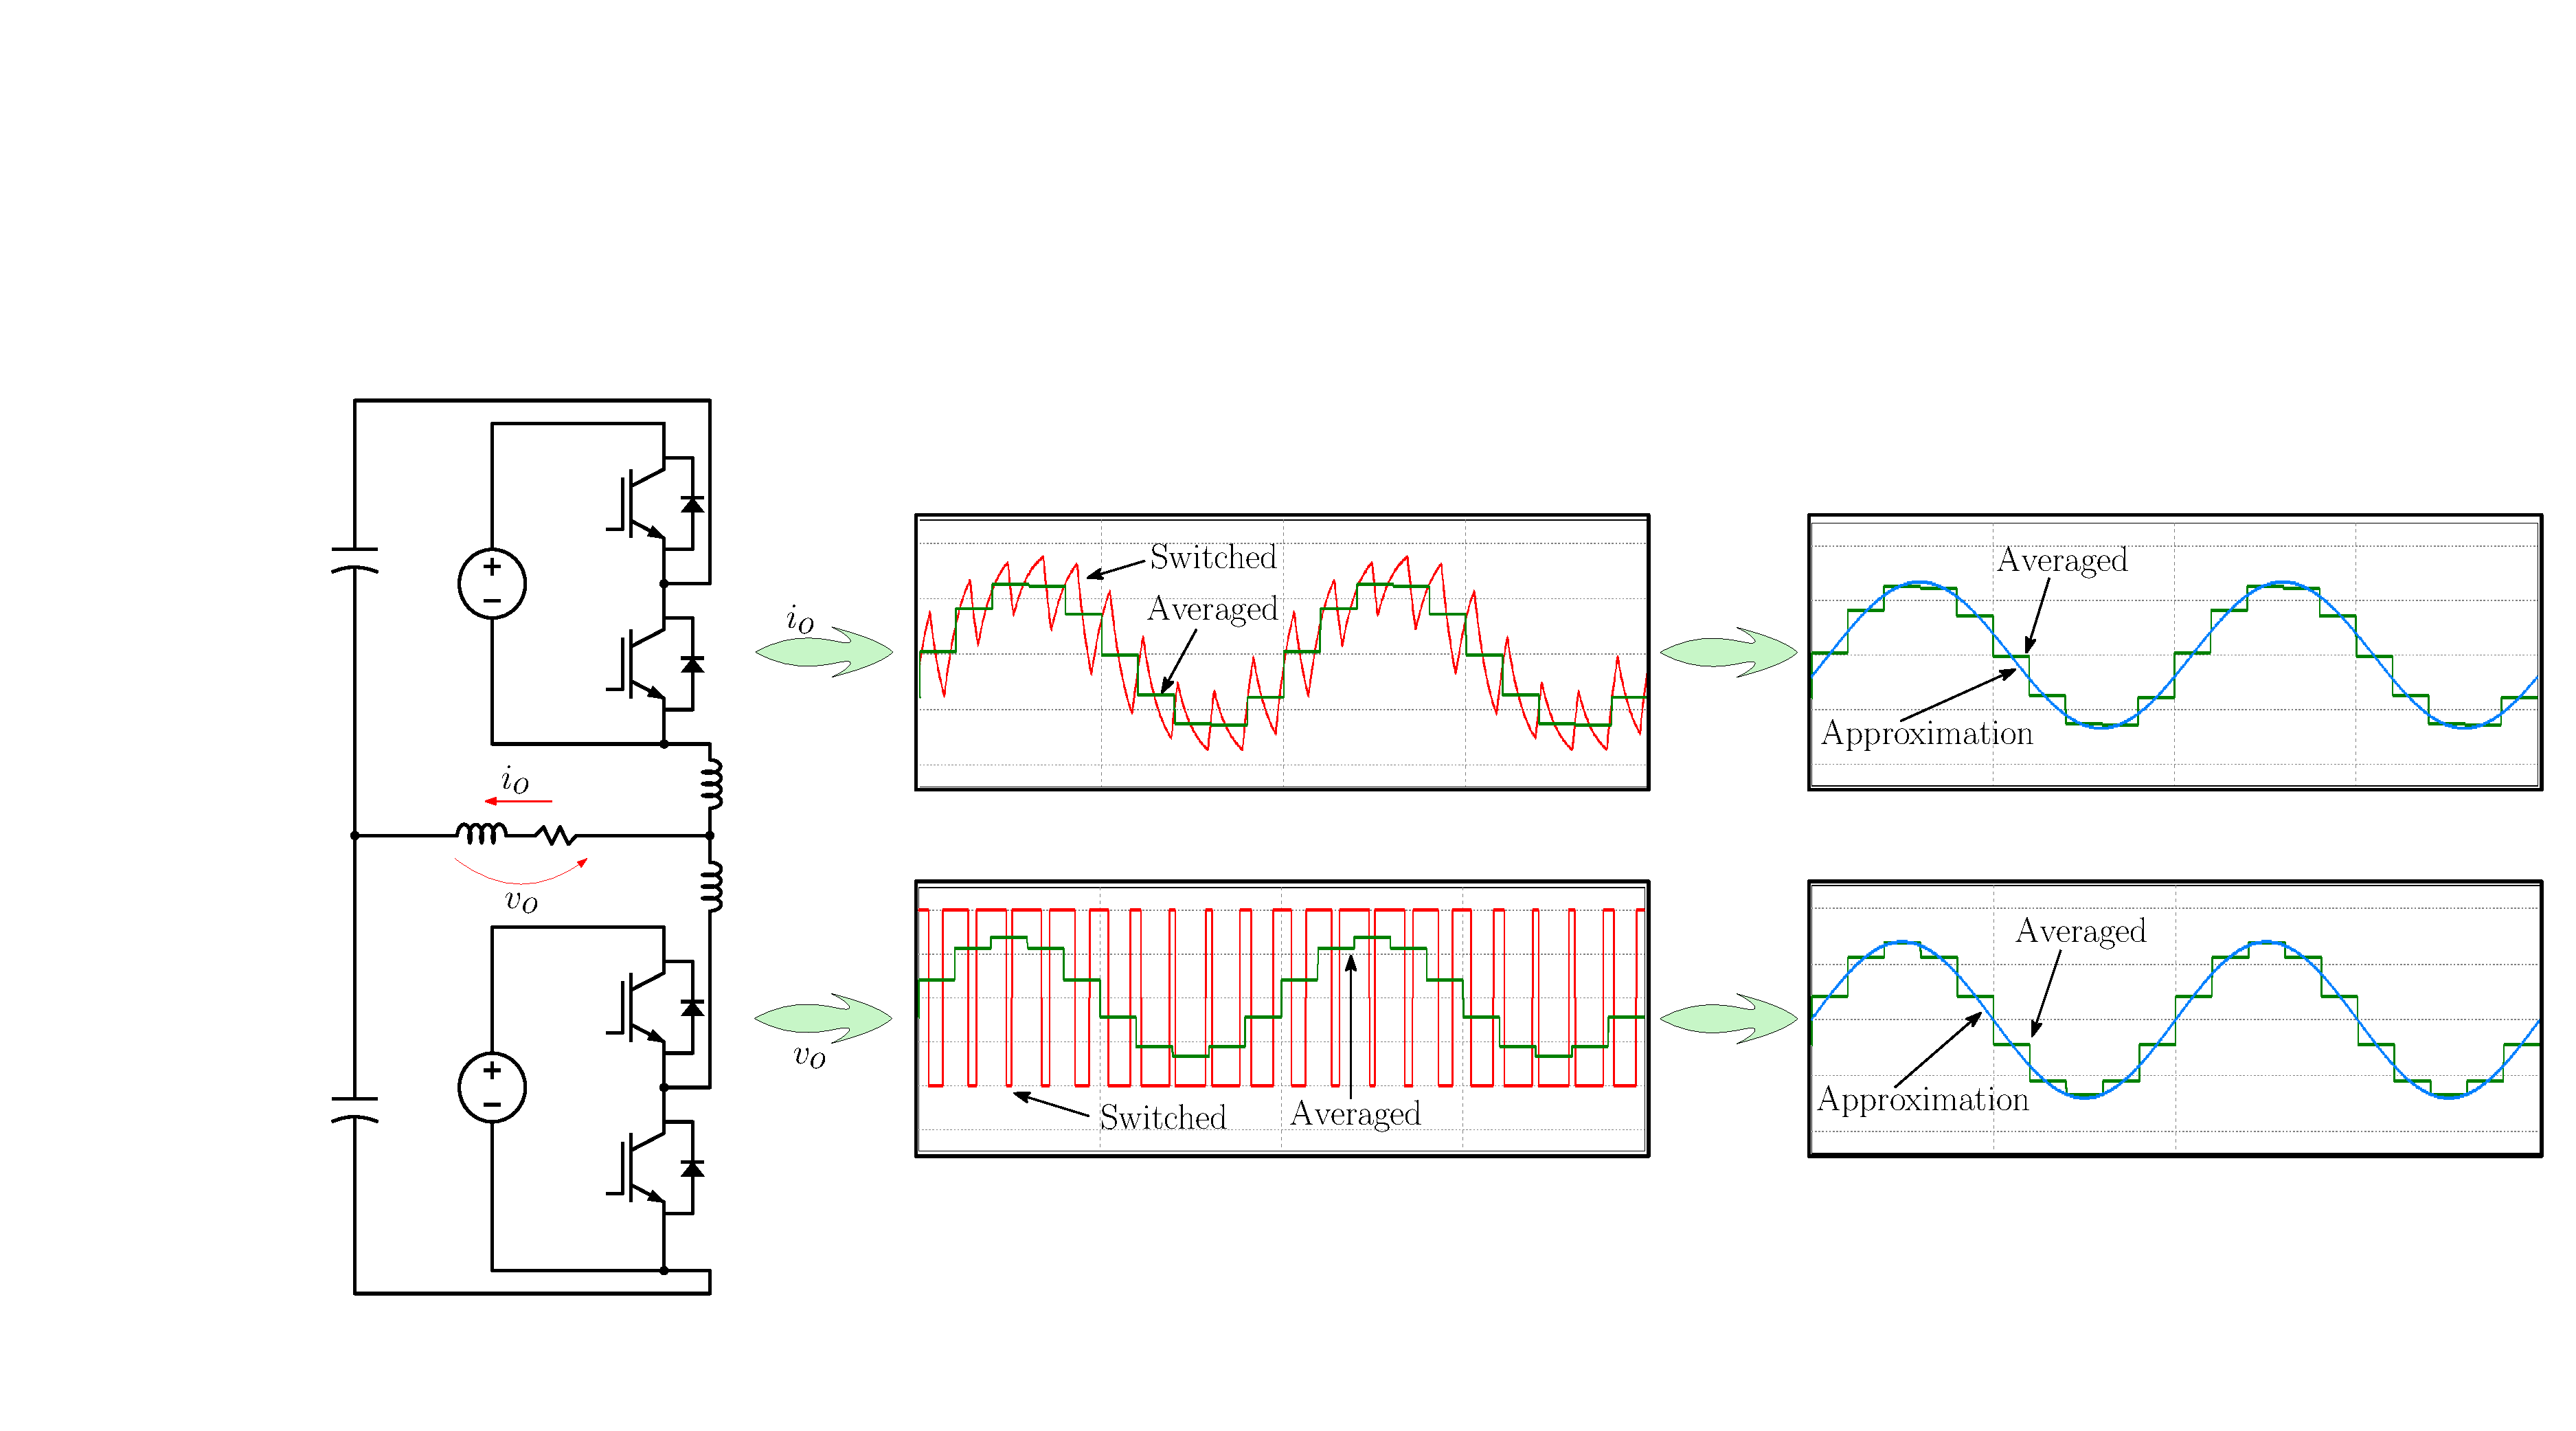
\includegraphics[width=0.9\linewidth]{./figuras/figuras_avg/AVG_EXPLAIN_2}
%
%\column{0.3\textwidth}
%
%
%\begin{itemize}
%	\item Desconsidera o efeito chaveamento
%	\item O padrão "escada" é aproximado por um comportamento contínuo
%\end{itemize}
%
%\end{columns}
%\vfill
%
%\begin{columns}
%
%
%\column{0.5\textwidth}
%\centering
%Tensão equivalente CA
%%
%\begin{equation*}
%v_{ac}^{pk}(t) = 
%m_p^k(t) v_{dc}^{pk}(t)
%\end{equation*}
%%
%\begin{equation*}
%v_{ac}^{nk}(t) = 
%m_n^k(t) v_{dc}^{nk}(t)
%\end{equation*}
%
%
%\column{0.5\textwidth}
%\centering
%
%Corrente equivalente CC
%%
%\begin{equation*}
%i_{dc}^{pk}(t) = m_{p}^{k}(t) i_{cp}^k(t)
%\end{equation*}    
%%
%\begin{equation*}
%i_{dc}^{nk}(t) = m_{n}^{k}(t) i_{cn}^k(t)
%\end{equation*}   
%
%\end{columns}
%
%
%\end{frame}
%







%%%%%%%%%%%%%%%%%%%%%%%%%%%%%%%%%%%%%%%%%%%%%%%%%%%%%%%
%%%%%%%%%%%%%%%%%%%%%%%%%%%%%%%%%%%%%%%%%%%%%%%%%%%%%%%
%%%%%%%%%%%%%%%%%%%%%%%%%%%%%%%%%%%%%%%%%%%%%%%%%%%%%%%
\begin{frame}{Modelo de Valor Médio}



\begin{columns}

\column{0.4\textwidth}

\centering
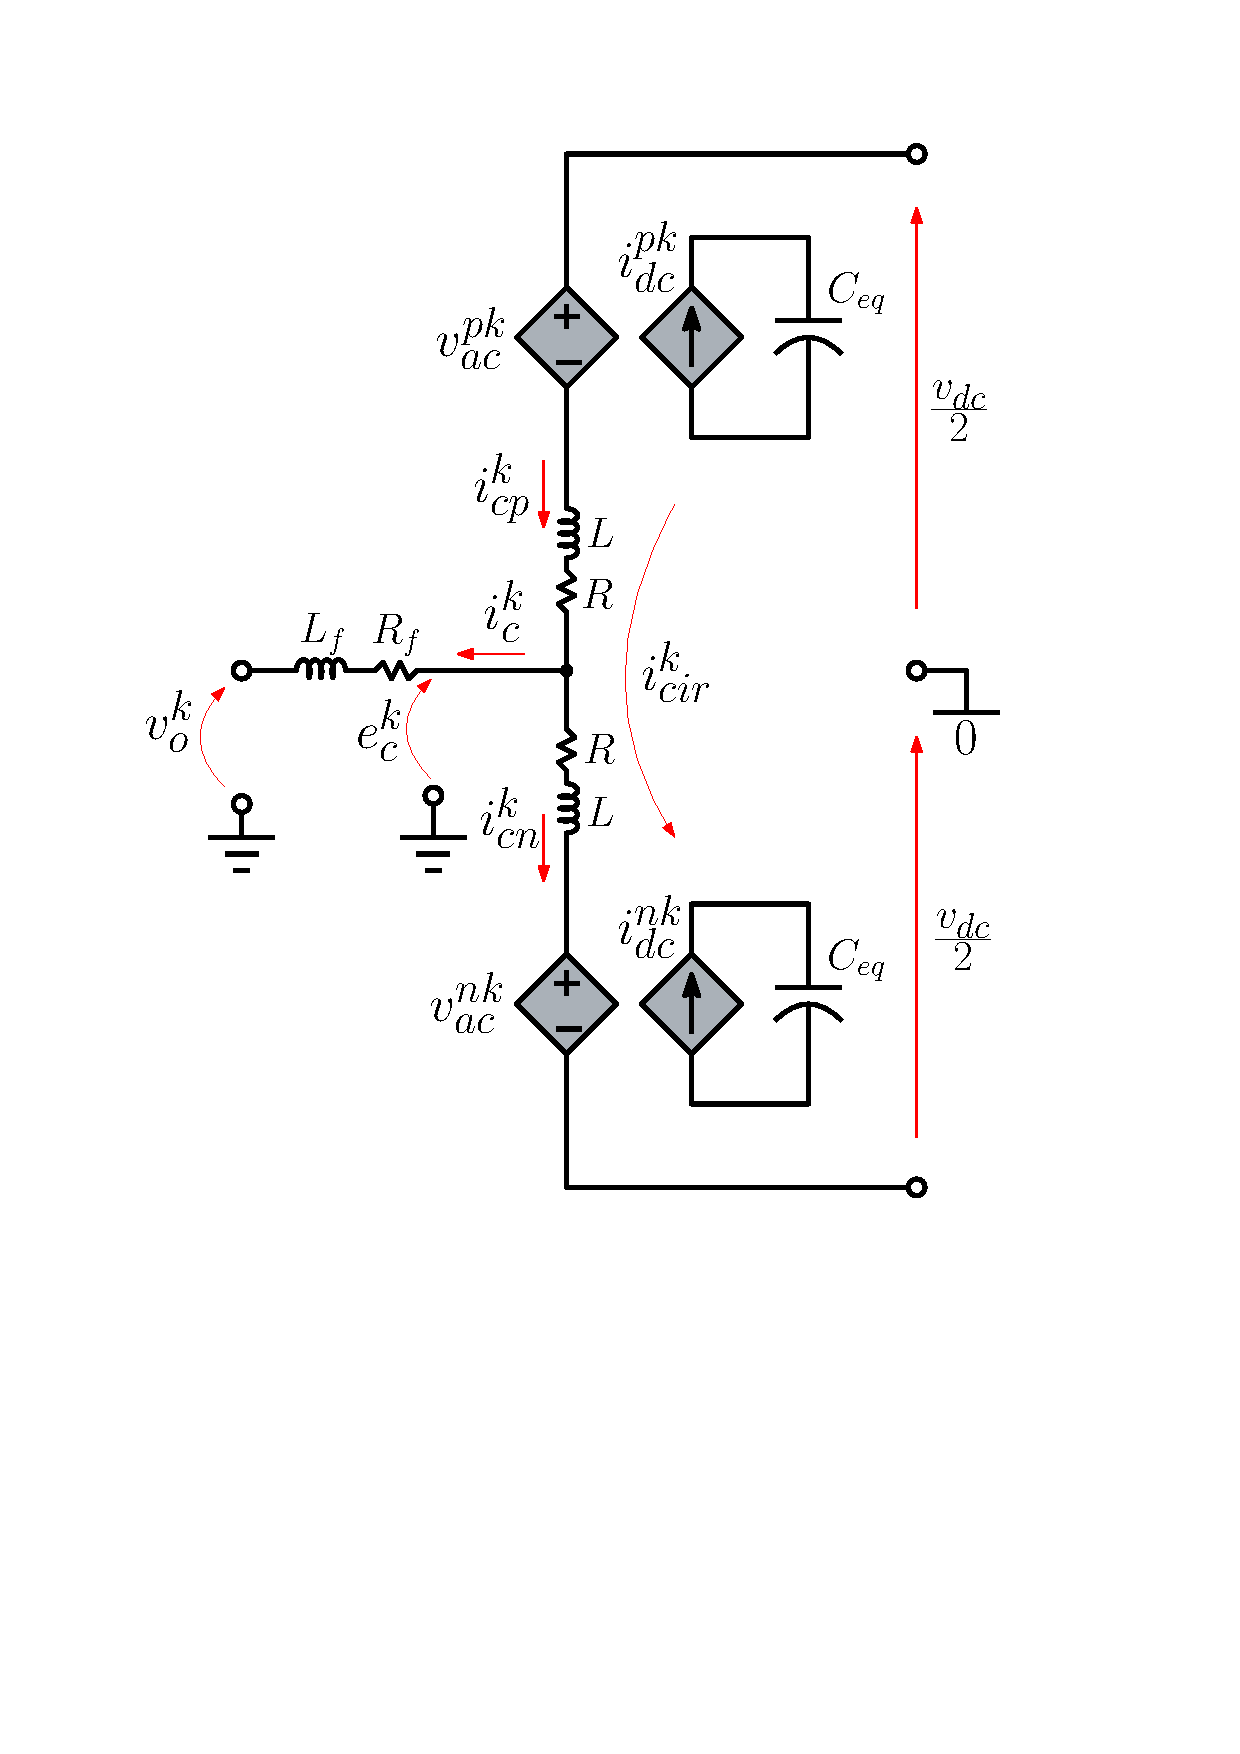
\includegraphics[width=0.9\linewidth]{./figuras/figuras_MMC/MMC_avg_2}

\column{0.3\textwidth}
\centering


\begin{itemize}
	\item Desconsidera o chaveamento\\[20pt]
	\item Fonte de tensão representa o lado CA dos SMs\\[20pt]
	\item Fonte de corrente representa o lado CC dos SMs
\end{itemize}

\column{0.3\textwidth}
\centering

Tensão equivalente CA
%
\begin{equation*}
v_{ac}^{pk}(t) = 
m_p^k(t) v_{dc}^{pk}(t)
\end{equation*}
%
\begin{equation*}
v_{ac}^{nk}(t) = 
m_n^k(t) v_{dc}^{nk}(t)
\end{equation*}\\[20pt]


Corrente equivalente CC
%
\begin{equation*}
i_{dc}^{pk}(t) = m_{p}^{k}(t) i_{cp}^k(t)
\end{equation*}    
%
\begin{equation*}
i_{dc}^{nk}(t) = m_{n}^{k}(t) i_{cn}^k(t)
\end{equation*}   

\end{columns}

\end{frame}


%%%%%%%%%%%%%%%%%%%%%%%%%%%%%%%%%%%%%%%%%%%%%%%%%%%%%%%
%%%%%%%%%%%%%%%%%%%%%%%%%%%%%%%%%%%%%%%%%%%%%%%%%%%%%%%
%%%%%%%%%%%%%%%%%%%%%%%%%%%%%%%%%%%%%%%%%%%%%%%%%%%%%%%
\begin{frame}{Modelo Não Linear}

Manipulando as equações de malha do circuito equivalente de valor médio:
\begin{multline*}
\resizebox{0.95\textwidth}{!} 
{$
\frac{d}{dt}\left[
\begin{array}{c}
i_{cir}^{k} \\[10pt] 
i_c^k  \\[10pt] 
v_{dc}^{k\Sigma}  \\[10pt] 
v_{dc}^{k\Delta} 
\end{array} 
\right]= 
\left[
\begin{array}{cccc}
-\frac{R}{L} & 0 & -\left(\frac{1-e_{cir}^{k*}}{4L}\right) & \frac{e_c^{k*}}{4L} \\[10pt] 
0 & -\left(\frac{R+2R_f}{L+2L_f}\right) & \frac{e_{c}^{k*}}{L+2L_f} & -\left(\frac{1-e_{cir}^{k*}}{L+2L_f}\right) \\[10pt] 
\frac{1-e_{cir}^{k*}}{C_{eq}} & -\frac{e_c^{k*}}{2C_{eq}} & 0 & 0 \\[10pt] 
-\frac{e_{c}^{k*}}{C_{eq}} & \frac{1-e_{cir}^{k*}}{2C_{eq}} & 0 & 0
\end{array} 
\right]
\left[
\begin{array}{c}
i_{cir}^{k} \\[10pt] 
i_c^k  \\[10pt] 
v_{dc}^{k\Sigma}  \\[10pt] 
v_{dc}^{k\Delta} 
\end{array}  
\right]+
\left[
\begin{array}{cc}
0 & \frac{1}{2L} \\[10pt] 
- \frac{2}{L+2L_f} & 0 \\[10pt] 
0 & 0 \\[10pt] 
0 & 0
\end{array} 
\right]
\left[
\begin{array}{c}
v_{o}^k \\[10pt] 
v_{dc} 
\end{array} 
\right] 
$}
\end{multline*}

onde:
\begin{equation*}
v_{dc}^{\Delta k}(t) = v_{dc}^{pk}(t) + v_{dc}^{nk}(t)
\end{equation*}
%
\begin{equation*}
v_{dc}^{\Sigma k}(t) = v_{dc}^{pk}(t) - v_{dc}^{nk}(t)
\end{equation*}




\end{frame}


%%%%%%%%%%%%%%%%%%%%%%%%%%%%%%%%%%%%%%%%%%%%%%%%%%%%%%%
%%%%%%%%%%%%%%%%%%%%%%%%%%%%%%%%%%%%%%%%%%%%%%%%%%%%%%%
%%%%%%%%%%%%%%%%%%%%%%%%%%%%%%%%%%%%%%%%%%%%%%%%%%%%%%%
\begin{frame}{Metodologia de Linearização}


Seja um sistema não linear com variáveis de estado $x$, de entrada $u$ e de perturbação $q$:

\begin{equation*}
\left\{
\begin{array}{l}
\dot{x}_1 = f_1(x_1,~\dots~,x_n,~u_1,~\dots~,u_m,~q_1,~\dots~,q_p)\\
\vdots\\
\dot{x}_n = f_n(x_1,~\dots~,x_n,~u_1,~\dots~,u_m,~q_1,~\dots~,q_p)
\end{array}
\right.
\end{equation*}


Sua representação linear é:
%
\begin{multline*}
\resizebox{0.95\textwidth}{!} 
{$
\left[
\begin{array}{c}
\dot{\tilde{x}}_1\\
\vdots\\
\dot{\tilde{x}}_n\\
\end{array}
\right] = 
\left[
\begin{array}{ccc}
\frac{\partial f_1}{\partial x_1} & \dots & \frac{\partial f_1}{\partial x_n}\\
\vdots & \ddots & \vdots\\
\frac{\partial f_n}{\partial x_1} & \dots & \frac{\partial f_n}{\partial x_n}
\end{array}
\right]
\left[
\begin{array}{c}
{\tilde{x}}_1\\
\vdots\\
{\tilde{x}}_n\\
\end{array}
\right] +
\left[
\begin{array}{ccc}
\frac{\partial f_1}{\partial u_1} & \dots & \frac{\partial f_1}{\partial u_m}\\
\vdots & \ddots & \vdots\\
\frac{\partial f_n}{\partial u_1} & \dots & \frac{\partial f_n}{\partial u_m}
\end{array}
\right]
\left[
\begin{array}{c}
{\tilde{u}}_1\\
\vdots\\
{\tilde{u}}_m\\
\end{array}
\right]+
\left[
\begin{array}{ccc}
\frac{\partial f_1}{\partial q_1} & \dots & \frac{\partial f_1}{\partial q_p}\\
\vdots & \ddots & \vdots\\
\frac{\partial f_n}{\partial q_1} & \dots & \frac{\partial f_n}{\partial q_p}
\end{array}
\right]
\left[
\begin{array}{c}
{\tilde{q}}_1\\
\vdots\\
{\tilde{q}}_p\\
\end{array}
\right]
$}
\end{multline*}

onde:

$\tilde{x}_n = x - x_{n0}$ ~~~~ $\tilde{u}_m = u - u_{m0}$ ~~~~ $\tilde{q}_n = q - q_{p0}$




\end{frame}



%%%%%%%%%%%%%%%%%%%%%%%%%%%%%%%%%%%%%%%%%%%%%%%%%%%%%%%
%%%%%%%%%%%%%%%%%%%%%%%%%%%%%%%%%%%%%%%%%%%%%%%%%%%%%%%
%%%%%%%%%%%%%%%%%%%%%%%%%%%%%%%%%%%%%%%%%%%%%%%%%%%%%%%
\begin{frame}{Modelo Linearizado}

Em referencial natural, temos:


\begin{equation*}
2 C_{eq} \frac{d \tilde{v}_{dc}^{\Sigma k}}{dt}(t) = 
2 \tilde{i}_{cir}^{k}(t) 
- \frac{2 S_0}{3 V_{dc0}} \tilde{e}_{cir}^{k*}(t)
\end{equation*}
%
\begin{equation*}
2 C_{eq}  \frac{d \tilde{v}_{dc}^{\Delta k}}{dt}(t) = 
- \frac{2 S_0}{3 V_{dc0}} \tilde{e}_c^{k*}(t) 
+ \tilde{i}_c^{k}(t)
\end{equation*}
%
\begin{equation*}
4 L \frac{d \tilde{i}_{cir}^{k}}{dt}(t) = 
- 4R \tilde{i}_{cir}^{k}(t)
- \tilde{v}_{dc}^{\Sigma k}(t) +  
2V_{dc0} \tilde{e}_{cir}^{k*}(t) 
+ 2  \tilde{v}_{dc}(t)
\end{equation*}
%
\begin{equation*}
 2\left( L + 2 L_f \right)  \frac{d \tilde{i}_c^k}{dt}(t) =   
 +  2V_{dc0}\tilde{e}_c^{k*}(t) -
  \tilde{v}_{dc}^{\Delta k}(t)  
 - 4 \tilde{v}_o^k(t) 
- 2\left(R + 2 R_f \right) \tilde{i}_c^k(t)
\end{equation*}




\end{frame}